%\documentclass[rnd]{mas_proposal}
\documentclass[thesis]{mas_proposal}

\usepackage[utf8]{inputenc}
\usepackage{amsmath}
\usepackage{amsfonts}
\usepackage{amssymb}
\usepackage{graphicx}
\usepackage{booktabs}
\usepackage{float}

\usepackage{lipsum}
\usepackage{array}
\usepackage{makecell}

\renewcommand\theadalign{bc}
\renewcommand\theadfont{\bfseries}
\renewcommand\theadgape{\Gape[4pt]}
\renewcommand\cellgape{\Gape[4pt]}



\usepackage{xcolor}
\usepackage{listings}
\usepackage{caption}
\DeclareCaptionFont{white}{\color{white}}
\DeclareCaptionFormat{listing}{%
	\parbox{\textwidth}{\colorbox{gray}{\parbox{\textwidth}{#1#2#3}}\vskip-4pt}}
\captionsetup[lstlisting]{format=listing,labelfont=white,textfont=white}
\lstset{frame=lrb,xleftmargin=\fboxsep,xrightmargin=-\fboxsep}

\lstset{
	% numbers=left,
	breaklines=true,
	% backgroundcolor=\color{light-gray},
	tabsize=4,
	% basicstyle=\ttfamily,
	literate={\ \ }{{\ }}1	
}

\title{Compliant Manipulation with Reinforcement Learning Guided by Task Specification}
\author{Abhishek Padalkar}
\supervisors{Prof. Dr. Paul G. Pl\"{o}ger\\Prof. Dr.-Ing. Gerhard K. Kraetzschmar \\Sven Schneider}
\date{\today}

% \thirdpartylogo{path/to/your/image}

\begin{document}

\maketitle

\pagestyle{plain}

\chapter{Introduction}
Most of the real world robotic manipulation tasks present the need for compliant manipulation, where robot needs to respond to the contact forces while executing the task. Classical planning and control algorithms fail to perform satisfactorily due to the lack of precise models of contact forces and high computational complexity. Various approaches have been proposed to learn compliant manipulation skills with the help of Reinforcement Learning (RL). RL is promising when it comes to learn intelligent behaviors in complex environments with high dimensions. But it requires high number of interactions with environment. In reinforcement learning, an agent learns the skills by exploring the environment and adopting the parameters which governs the trajectory of the agent in the environment. Learning all the parameters of the policy can be computationally very expensive and might require large number of interactions with the environment. Application of RL to robotics is limited by above reason. 

On the other hand, task specification approaches, proposed in \cite{leidner2017cognitive,mason1981compliance,bruyninckx1996specification} rely on instantaneous task specifications in task frames where constraint on motion are specified in each direction. Such approaches are more practical because of their deterministic nature which can be used for ensuring the robot's safe operation. But many parameters used in task specification need to be tuned manually which is a tedious task and requires number of human interventions. Moreover, sometimes, the task is too complex to be specified fully using task specification. 

Nemec et al. in \cite{nemec2017door} propose a control algorithm by joining reinforcement learning with intelligent control which learns force policy to open door on top of the specified motion for unlatching and opening door operation. We propose to extend above mentioned work by using task specification approach and using reinforcement learning for searching parameters good enough for executing the task maximizing a given reward function. Our approach combines the features from model based manipulation solutions and reinforcement learning. We propose to bring together the feature of deterministic solution from model based control solutions and self learning capability from reinforcement learning in one solution.  


\section{Problem Statement}
\begin{itemize}
	\item To develop a learning based approach for achieving compliant manipulation that allows to exploit partial/incomplete models
	of the task and the environment provided by the task specification.
	\item We plan to solve above problem by dividing the problem into two sub-problems:
	\begin{itemize}
		\item Model the available knowledge about task and environment using existing task specification framework.
		\item Use RL for learning gradually more complete and robust action models for compliant and repetitive manipulation tasks.
	\end{itemize}
    \item We will demonstrate our approach by learning a demo tasks of 
    \begin{itemize}
    	\item Opening door,
    	\item Cutting vegetables.
    \end{itemize}
\end{itemize}


\chapter{Related Work}
\section{Task specification}
In industrial settings, task are usually specified in the form of sequence of primitive motions\cite{leidner2017cognitive}. These motion primitives mostly contain point-to-point motion, motion to some default configuration and basic curves. For example, following script taken from KRL interface examples presents the motion primitives as shown in listing \ref{KRL-sample}. Though this kind of task specification works in controlled industrial environment, it leaves very little scope for external sensory feedback and the task needs to specified in terms of positional goals.

\begin{lstlisting}[label=KRL-sample,caption=KUKA Robot Language code]
INI
PTP HOME ; go to HOME joint configuration
LIN P1      ; linear motion to point P1
LIN P2	 ; linear motion to point P2
\end{lstlisting}

In \cite{leidner2017cognitive}, Leidner presented a representation in the form of action templates describing robot action using symbolic representations and geometric process model as shown in listing \ref{a-template}.  Symbolic representation of the task in PDDL allows classical planners to consider the action in the high level abstract task plan and geometric representation of the task specifies the sequence of low level movement sequences needed to complete the action. Here, geometric representation only specifies high level atomic motion primitives (e.g. \textit{move\_hand, move\_straight}) and not the parametric representation of the motion primitives. Actual parameterization and control is left to low level control module.   

\begin{lstlisting}[label=a-template,caption=Action Template: \_object.pick]
I Symbolic Representation 
'''(:action _object.pick: 
...
)'''

II Geometric Representation

def pick(self, manipulator, surface):
''' approach, grasp, and lift an object from a surface '''

graspset = odb.get_property(self.type, 'graspset', manipulator) 
for grasp_candidate in graspset: 
. . .
return operations
\end{lstlisting}

In \cite{mason1981compliance}, Mason et. al. presented the idea behind \textit{Task Frame Formalization - (TFF)} for specifying compliant task. Using hybrid control, various control specifying modes are assigned to each axis of the \textit{task frame} or \textit{compliance frame}\cite{nagele2018prototype}. Listing \ref{tff} shows Open Door task taken from \cite{bruyninckx1996specification}. This framework doesn't consider the specification of task quality or motion quality related parameters like velocity damping or instantaneous sensory inputs. 
\begin{lstlisting}[label=tff,caption=Task Specification using TFF: Open Door]
move compliantly {
	with task frame directions
	xt: force 0 N
	yt: force 0 N
	zt: velocity v mm/sec
	axt: force 0 Nmm
	ayt: force 0 Nmm
	azt: force 0 Nmm
} until distance > d mm 
\end{lstlisting}


iTaSC developed in \cite{DeSchutter-ijrr2007, DecreBruyninckxDeSchutter2013, decre09}, synthesizes control inputs based on provided task space constraints. It formulates a optimization problem considering provided constraints in the environment. In case of conflicting constraints, constraints are weighted in the optimization problem. 

\chapter{Reinforcement Learning}

Ideally, using reinforcement learning, an agent can find an optimal or near optimal behavior for a given reward function, by interacting with the environment. Instead of providing a detailed engineered solution, a reward function provides the feedback on the task which enables agent to learn a optimal solution.  

There are four major components in RL algorithm; policy, model, value function and reward function.

\section{Taxonomy in RL}

\textbf{Policy:}
A policy is a mapping from perceived states of the environment to actions to be taken when in those states. \\
\textbf{Model:}
Model mimics the behavior of the environment which allows agent to infer how environment will behave in response to a particular action. \\
\textbf{Value Function}
The value of a state is the total amount of reward an agent can expect to accumulate over the future, starting from that state. \\
\textbf{Reward Function}
Reward function is the feedback sent to the agent by the environment. It defines the goal of reinforcement learning problem.

A RL agent takes actions in the environment and receives feedback from the environment. Based on this feedback it learns a value function which gives the expected future return from that state. This value function is then used for building a policy for taking actions in the environment. 

Based on deployment of model of the environment, reinforcement learning approaches are categorized in two categories namely model-based and model-free reinforcement learning.


\section{Model Based Reinforcement Learning} \label{mod-RL}
In model based  reinforcement learning, the model of state transition dynamics is learned. This transition model is used for deriving rewards and value function. Policy for taking action is then derived from the value function. Value function in its simplest form, can be a table which stores all the state and value pairs and policy can be greedy search to take the action which will take the agent to the next state with highest value. But this approach heavily suffers from the accuracy of the transition dynamics model. This model is often learned in simulated environment, hence accuracy of simulation affects the accuracy of model being learned. So in short, we first model the world and use RL algorithms to learn this model of the world. Instead of this we can provide a incomplete parameterized model of the world and use RL to tune it.  


\section{Model Free Reinforcement Learning}

In model free reinforcement learning, no model of transition dynamics exist, hence value function and optimal actions are derived by trial and error\cite{polydoros2017survey}. In model free RL agent learns value function or policy or both (in actor-critic method) directly without learning model. Most of these trials are conducted in simulated environment. Hence the accuracy of simulation of the environment has significant impact on the value function and policy learned by the RL algorithm. The policy needs to be fine tuned in actual environment to compensate for the inaccurate or partially complete simulation.

\subsection{Policy search methods}
Application of reinforcement learning algorithm in robotics suffers from following problems \cite{deisenroth2013survey}:
\begin{itemize}
	\item high-dimensional continuous state and action spaces, 
	\item strong real- time requirements, and 
	\item the high costs of robot interactions with its environment.
\end{itemize} 
Policy search methods in RL bypass the learning of value function for policy generation, instead they learn the policy for action generation directly. Hence reinforcement learning problem involves only learning the policy parameters. Deisenroth et al. in \cite{deisenroth2013survey} present a comprehensive survey on policy learning in RL. According to this survey, widely used policy representations are: 1. Linear policies, 2. Radial basis function networks, 3. Dynamic motion primitives and 4. Miscellaneous representations. They also present survey on the methods used to learn this policies, which are: 1. policy gradients (PG), 2. expectation–maximization(EM)-based updates, and 3. information-theoretic insights.

Nemec et al. use reinforcement learning for learning force control policy for opening door\cite{nemec2017door}. They take into account the constraints on the door motion and closed kinematic chain resulting from a firm grasp of robot hand on the door handle. While opening the door in such configuration, high internal forces are generated in the direction where motion is not possible. They use this knowledge to learn a compliant force control policy. Our approach is motivated by this work of Nemec et al.\cite{nemec2017door}. We try to formalize constraints in terms of already existing task specification methods, which can be generalized to more number of compliant manipulation tasks. 

\section{Door Opening Task}

Opening door is one the most important task for service and rescue robots. Number of studies have been conducted to investigate this challenging problem using different techniques. Number of approaches rely on detail geometric modeling of the door and analytical trajectory generation. Nagatani et.al. \cite{nagatani1995experiment} presented an early approach for opening door by modeling the geometry of the door and then synthesizing trajectory to open door by considering geometrical constraints. To cope with the errors in position control of the early days manipulator used in the experiment, they used a force torque sensor module to achieve compliance with the environment. But this approach highly relies on correct geometric model and accurate execution of designed trajectories.

Approaches presented in \cite{levihn2014using,karayiannidis2012adaptive,niemeyer1997simple} use adaptive control algorithms which synthesize the motion by identifying the environmental constraints. In \cite{karayiannidis2012adaptive}, authors proposed to find the radial direction based on force and torque readings. Door is opened by applying velocity in radial direction. This method is prone to failure in case of uncertain grasp position. Also it considers only the case where door is already unlatched. 

Some of the methods for door opening motor primitives like Dynamic motion primitives for generating trajectories for opening door. Disadvantage of these approaches is that we need to know the goal pose to generate trajectory hence it confines the condition of completing the task to achieving a goal pose. 

\section{Vegetables Cutting Task}
Vegetable cutting task in an interesting problem for robot manipulation considering the complexity of contact forces. Different vegetables requires different cutting forces. Also force profile changes as we cut through the vegetables, e.g. tomato requires much less force once we cut through the skin. Such a complicated force interactions are very hard to model and specified in the task specification. Reinforcement learning provides the solution by allowing robots to learn force control policy over time or phase of the cutting task. This task was chosen for demonstration because of its complex contact force profile. Moreover the task itself does not need any external sensors other than force torque sensors to for estimating rewards and completion of the task.

In \cite{lioutikov2016learning}, Lioutikov et al. solved the task by learning Dynamic Motion Primitives, which is a trajectory control policy. Authors does not consider the problem as compliant manipulation problem hence contact forces are not taken into account. Task is solved just by performing Cartesian trajectory, and hence requiring multiple attempts to cut through the vegetable. 


\chapter{Proposed Solution}

We plan to solve a compliant manipulation task by providing a incomplete task specification and using Reinforcement Learning to determine un-modeled components in task specification. Provided task specification will greatly reduce the number of dimensions in reinforcement learning problem. And reinforcement learning will learn the parts in the task specification which is hard to model or tune.



\textbf{The outline proposed solution:}
\begin{itemize}
	\item Provide task specification using TFF, which also consists of parameters for the policy for generating control input.
	\item Provide policy for control command generation in the task specification (this policy can be a engineered policy for a custom solution or can be a generic parameterized policy e.g. neural network, radial basis function network, etc).
	\item Design a reward function for the given task.
	\item Use existing methods to adjust the parameters of the policy to maximize the reward function by carrying out trials in the environment.
\end{itemize}

\textbf{Advantages of proposed solution:}
\begin{itemize}
	\item Task specification models the available knowledge about the task which greatly reduces the dimensions of RL problem.
	\item An engineered policy for control input generation can be provided whenever possible. 
	\item Whenever it is not possible to engineer a policy, a generic policy can be used and limits on control inputs can be provided for ensuring robot's safe operation.
	\item Open parameters in policy provided in task specification can be learned using RL algorithm, which reduces human interventions and tedious manual parameter tuning. 

\end{itemize}

\section{Composition}

\begin{figure}[H]
	\center{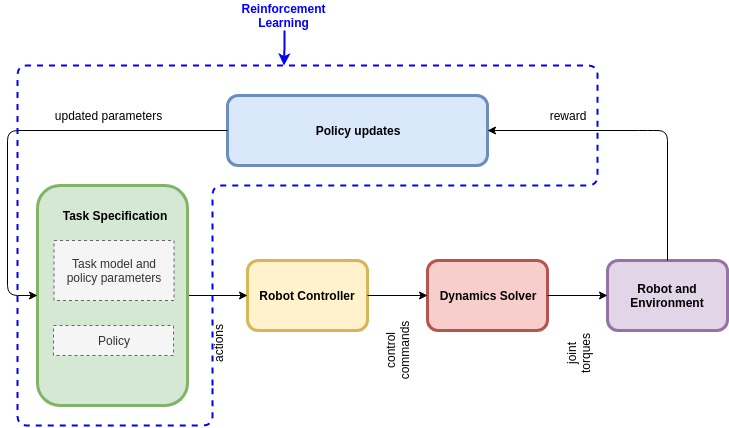
\includegraphics[width=\textwidth]
		{images/composition.png}}
	\caption{\label{fig:composition} Composition}
\end{figure}
Above figure shows the composition of the proposed solution.

\section{Task Specification}
We propose to use approach given by Mason et al.\cite{mason1981compliance}, with further modifications considering limitation on robot and environment. These parameters will also be used for ensuring quality of the task. e.g. smoothness in opening door. Also we introduce force and velocities as functions of robot and environmental parameters and phase of the task. 

\subsection{Examples of task specification:} 
\subsubsection{Opening door}

\begin{lstlisting}[label=open_door_ts,caption=Task specification for opening door]
open_door
{
	with task frame directions
	xt: force 0 N
	yt: force 0 N
	zt: velocity f(environment, robot, task) m/s
	axt: force 0 Nmm
	ayt: force 0 Nmm
	azt: force 0 Nmm
	max_acc = a_max m/ss
	max_dec = d_max m/ss
}until(g(...))

\end{lstlisting}
To understand the proposed solution, let's have detailed look at task of opening door. Door opening can be solved by applying velocity in tangential direction of door radius until it is opened till certain angle (different metrics of opened door can be brought in, here specified angle is chosen as it is generalizable for different situations). Robot arm needs to be compliant in other dimensions. Task specification given in Listing \ref{open_door_ts}, reflects this discussion. Here, task is formalized in door frame where z-axis is perpendicular to the door plane. To open the door smoothly, acceleration and deceleration should be limited. These parameters govern the trapezoidal shape of the velocity applied to door and those are identified as \textit{velocity policy parameters}. These open parameters, maximum acceleration and maximum deceleration, need to be tuned. Policy search methods in reinforcement learning can be deployed to find good enough parameters for maximizing a reward function which is designed to reduce the jerks in the motion and to reduce the time for opening as well.

In vegetable cutting task stated in Listing \ref{cut_vegies}, task is represented in chopping board frame such that z-axis is perpendicular to the chopping board and x-axis is in cutting direction. In this task, velocity in x-axis and force in z-axis are not easy to be modeled or parameterized. Here both of these entities can be represented by and generic parameterized policy. Moreover velocity can be learned from demonstrations using methods like Dynamic Motions Primitives\cite{lioutikov2016learning}. The advantage of the approach is clear here: control policy in only 2 dimensions out of 6 is to be learned because task specifications defines control inputs in other 4 dimensions. 

\begin{lstlisting}[label=cut_vegies,caption=Task specification for cutting vegetables]

cut_vegetables
{
	with task frame directions
	xt: velocity v(t) m/s
	yt: velocity 0 N
	zt: force f(environment, robot, task, xt) N
	axt: velocity 0 Nmm
	ayt: velocity 0 Nmm
	azt: velocity 0 Nmm
	max_acc = a_max m/ss
	max_dec = a_dec m/ss
}until(g(...))

\end{lstlisting}



\section{Reinforcement Learning Algorithm}

As already discussed, \begin{enumerate}
	\item Task specification approaches are reliable but they need manual tuning of many parameters.
	\item Sometimes force interactions in compliant manipulation tasks are so complex that parameterization of task and control policy is not possible. 
\end{enumerate}
Both of the above mentioned problems can be tackled by policy search methods in reinforcement learning. In first case, where an engineered control policy can be easily provided, reinforcement learning can be used for tuning policy parameters to maximize the given reward function.

Tasks where model parameterization is not possible, a generic parameterized policy can be used to learn the control policy. It is even possible to initialize this policy using learning from demonstration techniques.

In our case, we plan to represent control policy in terms of weighted Gaussian functions similar as in \cite{nemec2017door}. We plan to use Policy Improvement with Path Integral ($\text{PI}^{2}$) algorithm\cite{theodorou2010learning} for optimizing the policy parameters. ($\text{PI}^{2}$) is a sampling based algorithm which uses zero mean Gaussian noise to generate new parameters.   

\section{Robot Controller}

We propose to use robot specific impedance controller for controlling the robot. For KUKA LWR robot this controller is already provided by the manufacturer which is stated by following equation taken from \cite{schreiber2010fast}, an official documentation for KUKA Fast Research Interface.

\begin{equation}
\tau_{cmd} = J^{T}(K_{c}(x_{FRI} - x_{msr}) + D(d_{c}) + F_{FRI}) + f_{dynamics}(q, \dot{q}, \ddot{q})
\end{equation}

Where,
$\tau_{cmd}$ is commanded joint torque, $J$ is Jacobian of manipulator, $K_{c}$ is spring constant or stiffness constant, $x_{FRI}$ is commanded Cartesian position, $x_{msr}$ is current measured Cartesian position, $d_{c}$ is Cartesian normalized damping parameter, $F_{FRI}$ is commanded Cartesian force vector. The terms for the damping design $D(d_{c})$ and the dynamic model $f_{dynamics}(q, \dot{q}, \ddot{q})$ are taken care of in the KUKA motion
kernel.   

For manipulators which don't have internal torque controllers, but are equipped with the wrist force-torque sensors, impedance control can be achieved by a linear PID feedback controller which in turn controls velocity of end effector to control force and torque at end effector. Here the feedback is force and torque measurements by wrist force torque sensor. Such force torque controller can be given by equation below:
\begin{align}
	v =& P \cdot f_{e} + I \cdot \int f_{e} + D \cdot \dot{f_{e}} \\
	f_{e} =& f_{desired} - f_{measured}
\end{align}   
Where, $v$ is velocity vector of end-effector. $P, I, D$ are the gains in PID controller. $f_{desired}$ and $f_{measured}$ are the desired and measured force vectors respectively. 

And the Impedance Controller can be given by following equation:
\begin{align}
	f_{desired} = K(P_{d} - P_{m}) + D_{i}(\dot{P_{m}})
\end{align}
Where, $K$ is stiffness, $P_{d}$ and $P_{m}$ are desired and measured positions respectively, $D_{i}$ is damping coefficient. 

\chapter{Project Plan}
Project plan for this master thesis is as follows:
\section{Work Packages and Milestones}

\begin{tabular}{|c|c|c|}

	\hline
	\multicolumn{2}{|c|}{\thead{Work Packages}} & \thead{Targeted date} \\
	\hline
	WP01 & Literature search & 10-05-2019 \\
	WP02 & Analysis of state of the art &  \\
	\textit{MS01} & \textit{Documentation of the state of the art} &  \\
	\hline 
	WP03 & Modeling demo tasks using task specification approach &  20-06-2019\\ 
	WP04 & Design and implementation of the robot controller &   \\
	\textit{MS02} & \textit{Implementing task specification approach for door opening} &  \\
	\hline
	WP05 & Integrating RL algorithm in task specification & 30-07-2019 \\ 
	WP06 & Design and implementation of RL algorithm &   \\
	\textit{MS03} & \makecell{\textit{Implementing task specification approach} \\ \textit{with RL for door opening task}} &  \\
	\hline
	WP06 & Extending implemented solution for vegetable cutting task & 10-09-2019 \\ 
	WP07 & Experimental evaluation of implemented algorithms &  \\
	\textit{MS03} & \makecell{\textit{Implementing task specification approach with} \\ \textit{RL for cutting vegetable task}} &  \\
	\hline
\end{tabular}



\section{Deliverables}
Deliverables of this project are as follows: 
\subsection{Minimum Viable}

\begin{itemize}
    \item Literature survey and analysis of the state of the art.
    \item Design and implementation of task specification framework with reinforcement learning.
    \item Demonstration of task specification framework for door opening task without using reinforcement learning.
\end{itemize}

\subsection{Expected}
\begin{itemize}
    \item Demonstration of task specification framework with reinforcement learning for door opening task.
\end{itemize}

\subsection{Desired}
\begin{itemize}
	\item Extending proposed approach for cutting vegetable task.
    \item Demonstration of task specification framework with reinforcement learning for vegetable cutting task.
\end{itemize}


\nocite{*}

\bibliographystyle{plainnat} % Use the plainnat bibliography style
\bibliography{bibliography.bib} % Use the bibliography.bib file as the source of references




\end{document}
